% !TEX program = xelatex
\documentclass{article}
\usepackage{ctex}
\usepackage{listings}
\usepackage{xcolor}
\usepackage{geometry}
\usepackage{indentfirst}
\usepackage{setspace}
\usepackage{amsmath}
\usepackage{graphicx}
\usepackage{float}
\usepackage{titlesec}
\usepackage{hyperref}
\usepackage{bookmark}
\geometry{a4paper,margin=1in}
\setlength{\parindent}{2em}
\onehalfspacing
\titleformat{\subsection}{\large}{}{0em}{}
\lstset{
    basicstyle=\ttfamily\small,
    numbers=none,
    keywordstyle=\color{black},
    commentstyle=\color{green!60!black},
    stringstyle=\color{black},
    breaklines=true,
    showstringspaces=false,
    frame=none,
    backgroundcolor=\color{gray!10},
    captionpos=b,
    columns=fullflexible,
    keepspaces=true
}
\begin{document}
% 封面
\begin{titlepage}
    \centering
    \vspace*{3cm}
    {\Huge\bfseries Week3实验报告\par}
    \vspace{10cm}
    \begin{tabular}{l l}
    班级： & \underline{\makebox[6cm]{\centering 25级计算机科学与技术}} \\[1em]
    学号： & \underline{\makebox[6cm]{\centering 25020007028}} \\[1em]
    姓名： & \underline{\makebox[6cm]{\centering 官靓颖}} \\[1em]
    任课老师： & \underline{\makebox[6cm]{\centering 周小伟}} \\[1em]
    日期： & \underline{\makebox[6cm]{\centering 2026年9月7日}}
    \end{tabular}
    \vfill
\end{titlepage}
% ========== 正文开始 ==========
\subsection{\url{https://github.com/guan-111/Fundamentals-of-System-Development-Tools-Week3} }
 \begin{figure}[H]
     \centering
    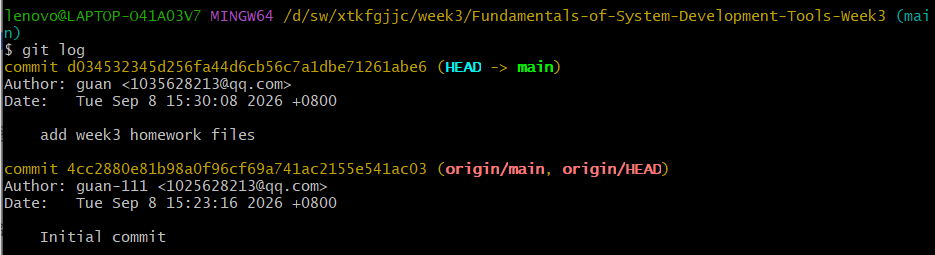
\includegraphics[width=0.7\textwidth]{commit.png}
     \caption{COMMIT}
     \label{fig:commit}
 \end{figure}




\section*{第一部分：实验习题}
\subsection*{第一题：从源码构建并在干净环境安装 Wheel}
\paragraph{主题：Packaging and Shipping Code}
\paragraph{在 q09 中按给定内容创建一个最小 Python 命令行包，并验证 wheel 安装。}
\paragraph{给定内容}
\begin{lstlisting}
# src/greetlab/cli.py
import argparse
def main():
    p = argparse.ArgumentParser()
    p.add_argument("--name", required=True)
    a = p.parse_args()
    print(f"Hello, {a.name}!")
# pyproject.toml
[build-system]
requires = ["setuptools>=68"]
build-backend = "setuptools.build_meta"
[project]
name = "greetlab-学号"
version = "0.1.0"
[project.scripts]
sdt-greet = "greetlab.cli:main"
\end{lstlisting}
\subsubsection*{1.创建 src/greetlab/\_\_init\_\_.py、给定的 cli.py 和 pyproject.toml，并把“学号”替换为自己的学号。}
 \begin{figure}[H]
     \centering
    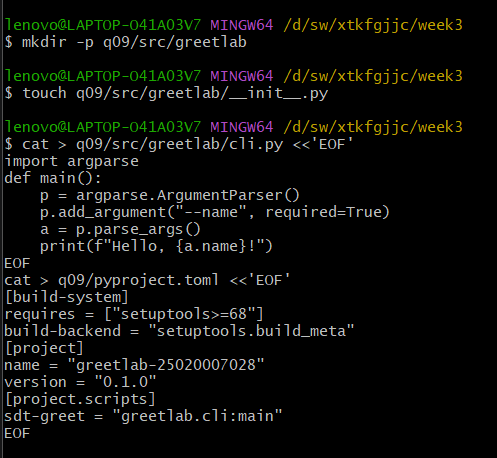
\includegraphics[width=0.7\textwidth]{0901.png}
     \caption{0901}
     \label{fig:q09_01}
 \end{figure}

\paragraph{知识点：}
\begin{enumerate}
\item \texttt{src}布局：Python现代包源码放置在src目录下，避免源码被意外直接导入。
\item \texttt{\_\_init\_\_.py}标记目录为Python包；现代pyproject.toml是标准项目元配置文件，替代旧版setup.py。
\item \texttt{[project.scripts]}定义命令行入口，将脚本命令映射到包内函数\texttt{模块:函数}。
\end{enumerate}
\subsubsection*{2. 在已安装 build 工具的课程环境中运行 python -m build，生成 wheel。}
 \begin{figure}[H]
     \centering
     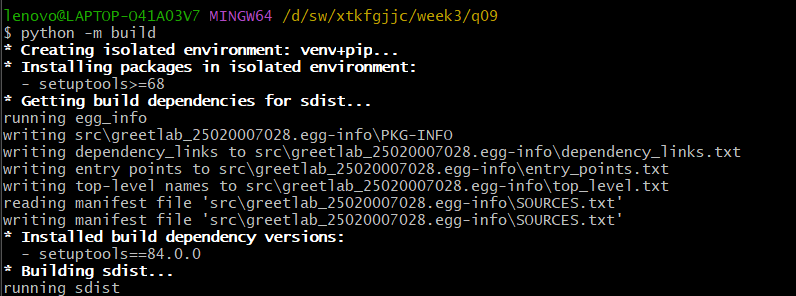
\includegraphics[width=0.7\textwidth]{090201.png}
     \caption{090201}
     \label{fig:q09_02}
 \end{figure}

 \begin{figure}[H]
     \centering
     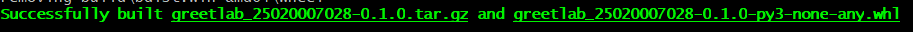
\includegraphics[width=0.7\textwidth]{090202.png}
     \caption{090202}
     \label{fig:q09_02}
 \end{figure}

\paragraph{知识点：}
\begin{enumerate}
\item \texttt{python -m build}：Python官方构建工具，在隔离环境构建源码包sdist与wheel二进制包。
\item wheel（*.whl）是预构建分发格式，安装速度比sdist源码包更快，不需要本地编译。
\item build会自动创建dist目录，产物sdist、wheel输出到dist文件夹。
\end{enumerate}
\subsubsection*{3.新建一个干净虚拟环境，只从生成的 wheel 安装。}
 \begin{figure}[H]
    \centering
     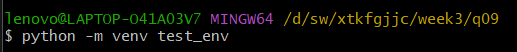
\includegraphics[width=0.7\textwidth]{090301.png}
     \caption{090301}
     \label{fig:q09_03}
 \end{figure}

 \begin{figure}[H]
    \centering
     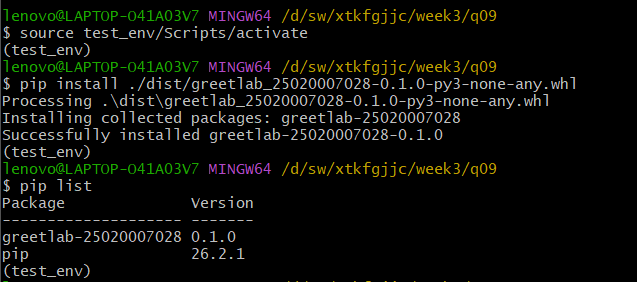
\includegraphics[width=0.7\textwidth]{090302.png}
     \caption{090302}
     \label{fig:q09_03}
 \end{figure}

\paragraph{知识点：}
\begin{enumerate}
\item \texttt{python -m venv} 创建隔离虚拟环境，不继承外部项目源码，只依靠安装包。
\item 从wheel安装：直接使用whl文件，不再读取src源码目录，验证打包产物完整性。
\item 干净环境用于验证：保证包运行只依赖pyproject.toml声明的依赖，不依赖本地环境残留文件。
\end{enumerate}
\subsubsection*{4.切换到 q09 之外运行 sdt-greet --name <学号>，确认输出正确。}
 \begin{figure}[H]
     \centering
     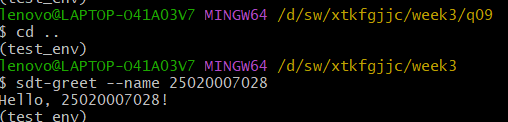
\includegraphics[width=0.7\textwidth]{0904.png}
     \caption{0904}
     \label{fig:q09_04}
 \end{figure}

\paragraph{知识点：}
\begin{enumerate}
\item 安装完成后\texttt{[project.scripts]}定义的命令 \texttt{sdt-greet} 被放置到虚拟环境bin目录，可以全局调用。
\item 在项目目录外部执行命令，验证包不是依赖本地src源码，而是真正完成安装。
\item argparse库用于快速编写命令行参数解析程序，\texttt{--name}为必填命令行参数。
\end{enumerate}
\subsection*{第二题：让编程智能体进入可验证的修复循环}
\paragraph{主题：智能体编程}
\paragraph{复用第9题的 greetlab 包，使用编程智能体完成一个小型测试驱动修复。}
\paragraph{给定内容}
\begin{lstlisting}
# 复用q09的greetlab包代码
# src/greetlab/cli.py
import argparse
def main():
    p = argparse.ArgumentParser()
    p.add_argument("--name", required=True)
    a = p.parse_args()
    print(f"Hello, {a.name}!")
\end{lstlisting}
\subsubsection*{1.复制q09为q10，添加一个失败测试：当name只含空白字符时，main应以SystemExit(2)结束。}
 \begin{figure}[H]
     \centering
     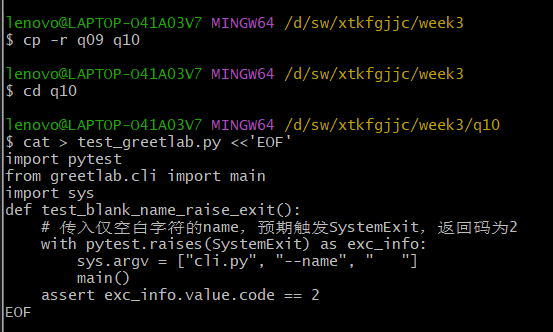
\includegraphics[width=0.7\textwidth]{100101.png}
     \caption{复制项目}
     \label{fig:q10_01}
 \end{figure}

  \begin{figure}[H]
     \centering
     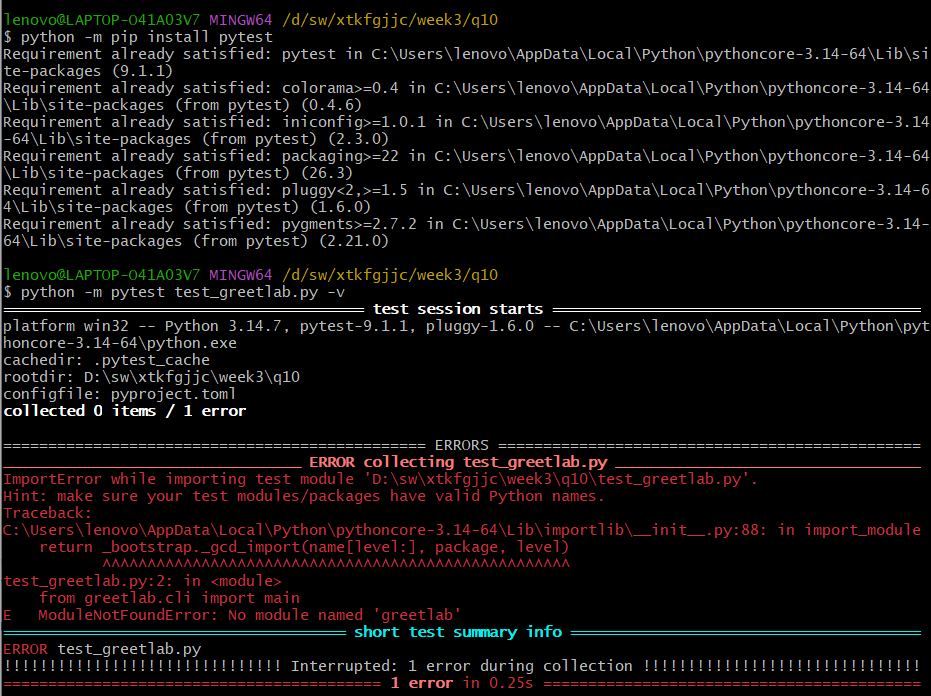
\includegraphics[width=0.7\textwidth]{100102.png}
     \caption{测试}
     \label{fig:q10_01}
 \end{figure}

\paragraph{知识点：}
\begin{enumerate}
\item 复制已有项目目录得到q10，基于已有包做增量开发，避免重复搭建项目结构。
\item \texttt{pytest.raises(SystemExit)}捕获程序退出异常，校验程序退出码，用于命令行程序测试。
\item 测试先行：先编写预期会失败的测试用例，确认当前实现不满足需求，这是测试驱动修复的起点。
\item \texttt{sys.argv}模拟命令行传入参数，不需要真实在终端输入命令即可测试cli入口函数。
\end{enumerate}
\subsubsection*{2.先运行测试确认失败，再向编程智能体说明目标、约束和测试命令，要求它修改实现并运行测试。}
 \begin{figure}[H]
     \centering
     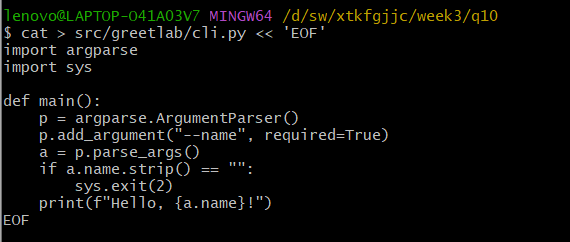
\includegraphics[width=0.7\textwidth]{100201.png}
     \caption{修改}
     \label{fig:q10_02}
 \end{figure}

\begin{figure}[H]
     \centering
     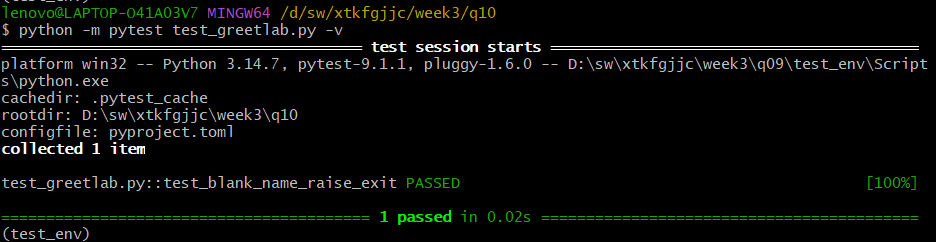
\includegraphics[width=0.7\textwidth]{100202.png}
     \caption{测试}
     \label{fig:q10_02}
 \end{figure}


\begin{lstlisting}
智能体任务提示：
目标：修改cli.py的main函数，如果--name传入的值仅由空白字符构成，以SystemExit(2)退出。
约束：不要改动其他逻辑，保留原有打印逻辑；使用已有的argparse，不要修改pyproject.toml；修复完成后运行pytest test_greetlab.py验证。

\end{lstlisting}
\paragraph{知识点：}
\begin{enumerate}
\item 可验证智能体修复循环：先有失败测试作为判定标准，智能体依据明确目标+约束修改源码，再执行测试做自动验证。
\item \texttt{sys.exit(n)}用于指定退出码结束程序；退出码2用来标识输入参数非法。
\item 给智能体提示必须写清目标、约束、验证命令，减少无关改动，避免AI随意重构代码。
\end{enumerate}
\subsubsection*{3.人工检查 diff，撤销无关修改，并再次运行测试。}
 \begin{figure}[H]
     \centering
     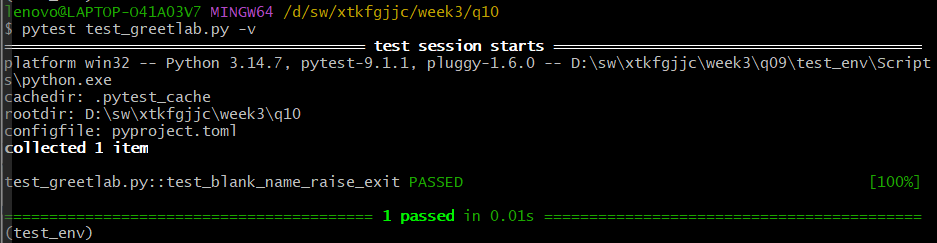
\includegraphics[width=0.7\textwidth]{1003.png}
     \caption{重跑测试}
     \label{fig:q10_03}
 \end{figure}

\paragraph{知识点：}
\begin{enumerate}
\item \texttt{git diff}查看文件改动，人工审查AI生成代码，过滤AI引入的多余、无关变更。
\item AI输出代码不一定最小修复，需要人工评审，只保留完成需求的最小改动。
\item 人工审查完成后再次运行测试，保证清理之后功能依旧正确。
\end{enumerate}
\subsubsection*{4.在 ai\_log.md 中用不超过5行记录核心提示、智能体改动和人工验证。}
 \begin{figure}[H]
     \centering
     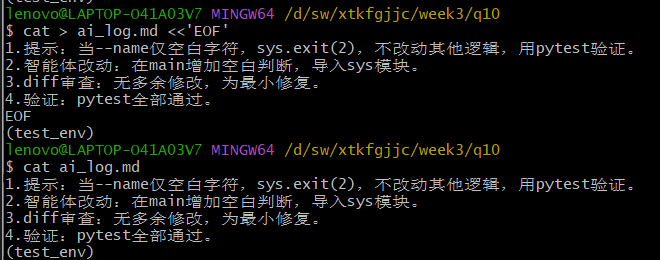
\includegraphics[width=0.7\textwidth]{1004.png}
     \caption{ai\_log.md日志记录}
     \label{fig:q10_04}
 \end{figure}

\paragraph{知识点：}
\begin{enumerate}
\item \texttt{ai\_log.md}记录智能体交互关键信息，留存修复过程证据。
\item 记录保持简短，聚焦：提示词、代码改动点、人工审查结果、测试验证结果。
\item 完整闭环：编写测试→AI修复→人工diff审查→回归测试→过程留档。
\end{enumerate}

\subsection*{第三题：把“无法处理”的协作材料改成可执行信息}
\paragraph{主题：不止于代码}
\paragraph{围绕“空姓名仍输出问候语”这一缺陷，改写下面三段质量较差的协作材料。}
\paragraph{给定内容}
\begin{lstlisting}
Issue: Windows 上运行不了，尽快修复。
提交信息: fix bug
评审意见: 这里写得不好，重写。
已知事实: 运行 sdt-greet --name "   " 时仍输出 Hello,  !，并以 0 退出。
\end{lstlisting}

\begin{figure}[H]
    \centering
    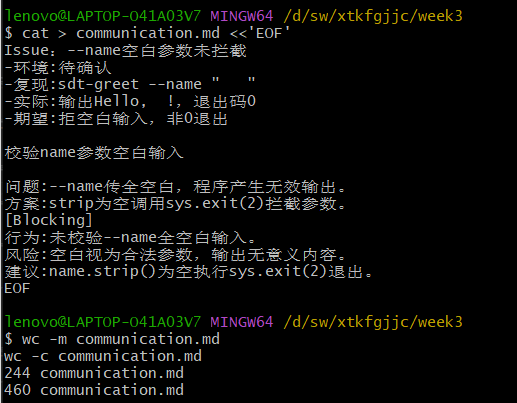
\includegraphics[width=0.7\textwidth]{1102.png}
    \caption{重写Issue内容}
    \label{fig:q11_01}
\end{figure}

\subsubsection*{1.在 communication.md 中重写 Issue，包含环境、复现命令、期望结果和实际结果；未知信息写“待确认”。}

\begin{lstlisting}
Issue：--name空白参数未拦截
-环境:待确认
-复现:sdt-greet --name "   "
-实际:输出Hello,  !，退出码0
-期望:拒空白输入，非0退出
\end{lstlisting}
\paragraph{知识点：}
\begin{enumerate}
\item 高质量Issue需要写明运行环境、复现步骤、实际现象、预期行为，便于他人复现定位bug。
\item 信息不确定处填写“待确认”，不做无依据猜测；避免模糊描述如“运行不了，尽快修复”。
\item 把客观现象和主观推测分开记录，只陈述观察到的程序输出与退出码。
\end{enumerate}

\subsubsection*{2.重写提交信息：标题使用祈使语气，正文说明问题和解决方案。}

\begin{lstlisting}
校验name参数空白输入

问题:--name传全空白，程序产生无效输出。
方案:strip为空调用sys.exit(2)拦截参数。
\end{lstlisting}
\paragraph{知识点：}
\begin{enumerate}
\item Git提交信息标题采用祈使句（动词开头），不要写“fixed bug”这类模糊描述。
\item 提交正文简短说明：是什么问题、本次改动如何解决该问题；标题与正文之间保留空行。
\item 拒绝 “fix bug”这种无信息量提交，便于后续查阅版本历史理解改动意图。
\end{enumerate}

\subsubsection*{3.重写评审意见：指出具体行为、风险和建议动作，并标注Blocking、Suggestion或Nit。}

\begin{lstlisting}
[Blocking]
行为:未校验--name全空白输入。
风险:空白视为合法参数，输出无意义内容。
建议:name.strip()为空执行sys.exit(2)退出。
\end{lstlisting}
\paragraph{知识点：}
\begin{enumerate}
\item Blocking：必须修改，否则不能合并；Suggestion：建议修改，可以酌情考虑；Nit：小瑕疵，可直接合并。
\item 评审意见不能笼统说“写得不好重写”，要指出具体行为、带来什么风险、给出明确修改动作。
\item 协作沟通面向事实，给出可执行的修改指引，减少沟通歧义。
\end{enumerate}

\subsubsection*{4.全文控制在400字以内，保持专业、简洁。}

\begin{lstlisting}
# wc -m 统计逻辑字符数，确认总字符小于400
wc -m communication.md
# wc -c 统计字节数，受中文编码影响，不作为字数判断依据
wc -c communication.md
\end{lstlisting}
\paragraph{知识点：}
\begin{enumerate}
\item 技术协作文档力求简洁，去掉冗余抒情，只保留客观事实、指令；控制篇幅便于快速阅读。
\item \texttt{wc -m}统计逻辑字符，每个汉字、符号计为1个；\texttt{wc -c}统计磁盘字节，中文会占用多个字节，不能用来判断“字数”。
\item 模糊、情绪化描述会提升团队沟通成本，可执行的书面材料是高效协作的基础。
\item Issue、commit message、code review三者共同构成项目可追溯的协作证据链。
\end{enumerate}

\subsection*{第四题：修复一个可复现的线性回归训练循环}
\paragraph{主题：Python与PyTorch}
\paragraph{将下方代码保存为 q12/train.py，补全TODO并完成一次 PyTorch CPU 训练。}
\paragraph{给定内容}
\begin{lstlisting}
import torch
from torch import nn
torch.manual_seed(20260907)
x = torch.linspace(-1, 1, 101).reshape(-1, 1)
y = 3 * x - 1
model = nn.Linear(1, 1)
loss_fn = nn.MSELoss()
opt = torch.optim.SGD(model.parameters(), lr=0.1)
for _ in range(200):
    pred = model(x)
    loss = loss_fn(pred, y)
    # TODO: 清空梯度、反向传播、更新参数
# TODO: 进入评估模式并在no_grad中打印最终损失、weight和bias
\end{lstlisting}
\subsubsection*{1.补全训练循环，正确调用 zero\_grad、backward 和 step。}
 \begin{figure}[H]
     \centering
     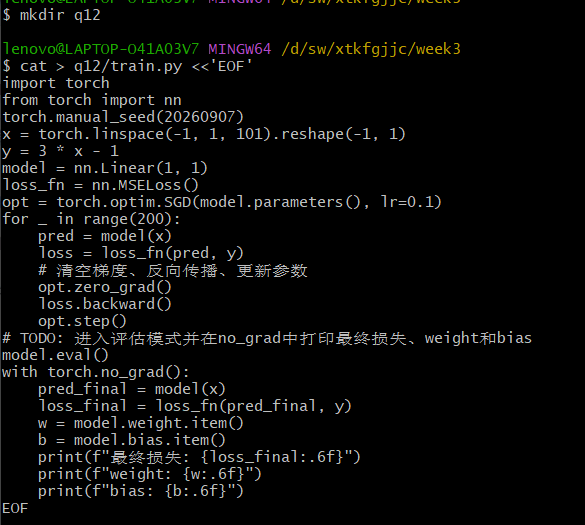
\includegraphics[width=0.7\textwidth]{120101.png}
     \caption{补全训练循环代码}
     \label{fig:q12_01}
 \end{figure}

\paragraph{知识点：}
\begin{enumerate}
\item \texttt{opt.zero\_grad()}：清空上一轮累积梯度，PyTorch梯度默认累加，每轮训练必须清零。
\item \texttt{loss.backward()}：反向传播，自动计算各参数梯度值。
\item \texttt{opt.step()}：优化器根据梯度更新模型参数，完成一轮参数迭代。
\item 训练循环标准顺序：前向计算→计算损失→清零梯度→反向传播→参数更新。
\end{enumerate}
\subsubsection*{2.训练后调用 model.eval()，并在 torch.no\_grad() 中计算最终损失。}
 \begin{figure}[H]
     \centering
     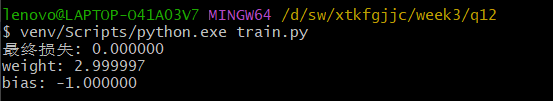
\includegraphics[width=0.7\textwidth]{120102.png}
     \caption{测试}
     \label{fig:q12_01}
 \end{figure}

\paragraph{知识点：}
\begin{enumerate}
\item \texttt{model.eval()}评估模式：关闭Dropout、BatchNorm等训练专用层行为，用于推理与测试。
\item \texttt{torch.no\_grad()}上下文管理器：禁用梯度计算，节省显存、加速运算，推理阶段必须使用。
\item 评估阶段不进行参数更新，不需要构建计算图，因此关闭梯度。
\end{enumerate}
\subsubsection*{3.打印最终损失、weight和bias；最终损失应小于0.001。}
 \begin{figure}[H]
     \centering
     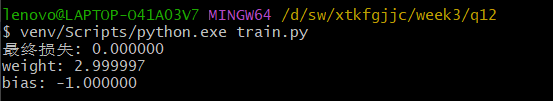
\includegraphics[width=0.7\textwidth]{120102.png}
     \caption{测试}
     \label{fig:q12_01}
 \end{figure}

\paragraph{知识点：}
\begin{enumerate}
\item \texttt{.item()} 将单元素tensor转为普通Python数值，方便打印输出。
\item MSELoss均方误差损失，训练充分后损失下降到0.001以下，权重逼近真实3，偏置逼近真实-1。
\item \texttt{torch.manual\_seed()}固定随机种子，保证实验结果可复现。
\end{enumerate}
\subsubsection*{4.不得直接把 weight 和 bias 赋值为 3 和 -1。}

\begin{lstlisting}
# 错误写法（禁止）
# model.weight[:] = 3
# model.bias[:] = -1
\end{lstlisting}
\paragraph{知识点：}
\begin{enumerate}
\item 实验要求依靠SGD优化器迭代训练得到参数，不允许直接写死标准答案。
\item 考察对完整训练流程理解，模拟真实机器学习任务，参数由数据与优化算法学习得到。
\item 即使已知解析解，仍然需要走完整前向‑损失‑反向‑更新训练闭环。
\end{enumerate}

\section*{第二部分 实验实例}
\subsection*{实例一：构建源码分发包sdist并查看包元信息}
% \begin{figure}[H]
%     \centering
%     \includegraphics[width=0.7\textwidth]{ex_01.png}
%     \caption{构建sdist源码包，查看元信息}
%     \label{fig:ex_01}
% \end{figure}
\begin{lstlisting}
cd q09
python -m build --sdist
# 解压sdist源码包查看pyproject.toml
tar -xf dist/greetlab-25020007028-0.1.0.tar.gz
cat greetlab-25020007028-0.1.0/pyproject.toml
\end{lstlisting}
\paragraph{知识点：}
\begin{enumerate}
\item \texttt{python -m build --sdist}只构建源码分发包，sdist包含全部源码文件。
\item sdist发布后用户本地环境会执行构建流程生成wheel，对构建依赖有要求。
\item 解压sdist可以校验发布出去的配置文件是否和本地源码一致。
\end{enumerate}
\subsection*{实例二：pip从本地wheel文件安装并查看脚本入口}
% \begin{figure}[H]
%     \centering
%     \includegraphics[width=0.7\textwidth]{ex_02.png}
%     \caption{pip安装wheel，查找生成的命令行脚本}
%     \label{fig:ex_02}
% \end{figure}
\begin{lstlisting}
python -m venv demo_env
source demo_env/bin/activate
pip install dist/greetlab_25020007028-0.1.0-py3-none-any.whl
pip show greetlab-25020007028
# 查找生成的命令脚本
ls demo_env/bin/ | grep sdt-greet
\end{lstlisting}
\paragraph{知识点：}
\begin{enumerate}
\item \texttt{pip show}查看已经安装包的元数据、版本、安装路径。
\item wheel安装完成后，pyproject.toml定义的scripts会生成可执行脚本放置在虚拟环境bin目录。
\item wheel安装不需要本地编译环境，安装速度优于sdist源码包。
\end{enumerate}
\subsection*{实例三：pytest测试捕获命令行不同退出码SystemExit}
% \begin{figure}[H]
%     \centering
%     \includegraphics[width=0.7\textwidth]{ex_03.png}
%     \caption{测试捕获不同SystemExit退出码}
%     \label{fig:ex_03}
% \end{figure}
\begin{lstlisting}
cat > test_exitcode.py <<'EOF'
import pytest
import sys
from greetlab.cli import main
def test_exit_code_2():
    sys.argv = ["cli.py", "--name", "   "]
    with pytest.raises(SystemExit) as exc:
        main()
    assert exc.value.code == 2
def test_exit_code_0():
    sys.argv = ["cli.py", "--name", "Student"]
    with pytest.raises(SystemExit) as exc:
        main()
    assert exc.value.code == 0
EOF
pytest test_exitcode.py -v
\end{lstlisting}
\paragraph{知识点：}
\begin{enumerate}
\item \texttt{pytest.raises}不仅可以捕获异常类型，还可以校验异常携带的参数，例如程序退出码。
\item 合法输入正常运行返回SystemExit(0)；参数非法约定返回非0退出码，例如2。
\item 使用sys.argv模拟命令行入参，不需要子进程即可完成cli函数单元测试。
\end{enumerate}
\subsection*{实例四：git diff筛选只查看py文件改动，过滤无关文本变更}
% \begin{figure}[H]
%     \centering
%     \includegraphics[width=0.7\textwidth]{ex_04.png}
%     \caption{git diff过滤，只查看python源码改动}
%     \label{fig:ex_04}
% \end{figure}
\begin{lstlisting}
# 只看py后缀文件的diff，过滤md等其他文件改动
git diff -- *.py
\end{lstlisting}
\paragraph{知识点：}
\begin{enumerate}
\item AI修改代码时经常改动文档、注释等无关文件，可以使用路径过滤只审查源码变更。
\item 人工评审AI代码，聚焦业务逻辑文件，快速定位真实修复点。
\item git diff可以指定文件后缀，缩小代码审查范围，提升评审效率。
\end{enumerate}
\subsection*{实例五：编写高质量Bug Issue：区分实际现象与推测猜想}
% \begin{figure}[H]
%     \centering
%     \includegraphics[width=0.7\textwidth]{ex_05.png}
%     \caption{编写规范Issue，区分事实和猜想}
%     \label{fig:ex_05}
% \end{figure}
\begin{lstlisting}
cat > demo_issue.md <<'EOF'
## Bug报告
复现命令：sdt-greet --name ""
实际现象：程序输出 Hello, !，退出码0。
推测猜想：参数校验逻辑缺失，空字符串没有拦截。
期望行为：拦截空字符串输入，退出码2终止程序。
EOF
cat demo_issue.md
\end{lstlisting}
\paragraph{知识点：}
\begin{enumerate}
\item Issue中严格区分：客观复现现象（事实）和对根因的猜想。
\item 不要把猜想当成确定事实写进bug记录，根因需要调试验证。
\item 提供完整复现命令，其他人可以一键复现问题。
\end{enumerate}
\subsection*{实例六：规范Git commit，对比劣质提交信息与标准提交信息}
% \begin{figure}[H]
%     \centering
%     \includegraphics[width=0.7\textwidth]{ex_06.png}
%     \caption{劣质commit和规范commit对比示例}
%     \label{fig:ex_06}
% \end{figure}
\begin{lstlisting}
# 劣质提交示例（禁止）
# git commit -m "change something, fix problem"
# 规范提交示例
"""
增加空字符串参数校验
问题：空字符串参数不会被拦截，输出无意义问候。
修复：判断name.strip()为空时sys.exit(2)拒绝输入。
"""
\end{lstlisting}
\paragraph{知识点：}
\begin{enumerate}
\item Git commit标题动词祈使句开头，简短描述改动行为。
\item commit正文说明：存在什么问题、本次改动如何修复。
\item 模糊的提交信息，会导致版本历史难以追溯，不利于团队协作。
\end{enumerate}
\subsection*{实例七：代码评审标记 Nit / Suggestion / Blocking 三种等级实践}
% \begin{figure}[H]
%     \centering
%     \includegraphics[width=0.7\textwidth]{ex_07.png}
%     \caption{三种评审标签实践示例}
%     \label{fig:ex_07}
% \end{figure}
\begin{lstlisting}
"""
[Blocking]
行为：没有处理空字符串输入。
风险：非法参数会生成错误输出。
建议：增加空白字符校验，sys.exit(2)退出。
[Suggestion]
建议：给错误输出增加stderr提示文本，方便用户理解报错。
[Nit]
小瑕疵：该行尾部多余空格，可以清理，不影响功能。
"""
\end{lstlisting}
\paragraph{知识点：}
\begin{enumerate}
\item Blocking：必须修改，否则不能合并；Suggestion：建议修改，可权衡；Nit：格式小瑕疵，可以直接合并。
\item 评审意见写清楚行为、风险、动作，避免模糊描述“写的不好重写”。
\item 分级评审可以区分问题严重程度，提升团队协作效率。
\end{enumerate}
\subsection*{实例八：PyTorch训练循环错误示范：忘记zero\_grad观察梯度累积现象}
% \begin{figure}[H]
%     \centering
%     \includegraphics[width=0.7\textwidth]{ex_08.png}
%     \caption{不执行zero‑grad造成梯度累积演示}
%     \label{fig:ex_08}
% \end{figure}
\begin{lstlisting}
# 错误片段，注释opt.zero_grad()
# for ...:
#     pred = model(x)
#     loss = loss_fn(pred,y)
#     # opt.zero_grad()
#     loss.backward()
#     opt.step()
# print(model.weight.grad)
\end{lstlisting}
\paragraph{知识点：}
\begin{enumerate}
\item PyTorch梯度会累加，不调用zero\_grad()梯度不断累积，参数更新完全异常。
\item 这是深度学习训练高频bug，训练循环标准顺序不能颠倒、不能遗漏。
\item debug时打印\texttt{tensor.grad}，可以观察梯度是否正常。
\end{enumerate}
\subsection*{实例九：model.train()与model.eval()切换对比演示}
% \begin{figure}[H]
%     \centering
%     \includegraphics[width=0.7\textwidth]{ex_09.png}
%     \caption{train与eval模式切换演示}
%     \label{fig:ex_09}
% \end{figure}
\begin{lstlisting}
model.train()
print(f"训练模式：{model.training}")
model.eval()
print(f"评估模式：{model.training}")
with torch.no_grad():
    out = model(x)
\end{lstlisting}
\paragraph{知识点：}
\begin{enumerate}
\item \texttt{model.training}布尔变量标记模型当前处于训练/评估模式。
\item train模式启用dropout等训练层；eval模式关闭，推理测试必须切换eval。
\item torch.no\_grad()只管关闭梯度计算，**不会改变模型train/eval状态，两者需要配合使用**。
\end{enumerate}
\subsection*{实例十：固定随机种子保证PyTorch实验可复现完整示例}
% \begin{figure}[H]
%     \centering
%     \includegraphics[width=0.7\textwidth]{ex_10.png}
%     \caption{固定随机种子，复现实验结果}
%     \label{fig:ex_10}
% \end{figure}
\begin{lstlisting}
import torch
# 固定随机种子
torch.manual_seed(20260907)
m1 = nn.Linear(1,1)
w1 = m1.weight.item()
torch.manual_seed(20260907)
m2 = nn.Linear(1,1)
w2 = m2.weight.item()
print(w1, w2)
# 两次权重数值完全一致
\end{lstlisting}
\paragraph{知识点：}
\begin{enumerate}
\item \texttt{torch.manual\_seed()}固定CPU随机数生成器种子，保证模型初始化结果一致。
\item 机器学习实验必须固定随机种子，否则每次运行结果不一样，无法复现实验。
\item 可复现性是实验、调试、AI智能体修复循环的基础前提。
\end{enumerate}
\end{document}
